% One-page map: separate vertices for the main transformations and normal forms.
\begin{figure}[p]
\centering
\resizebox{!}{.82\textheight}{%
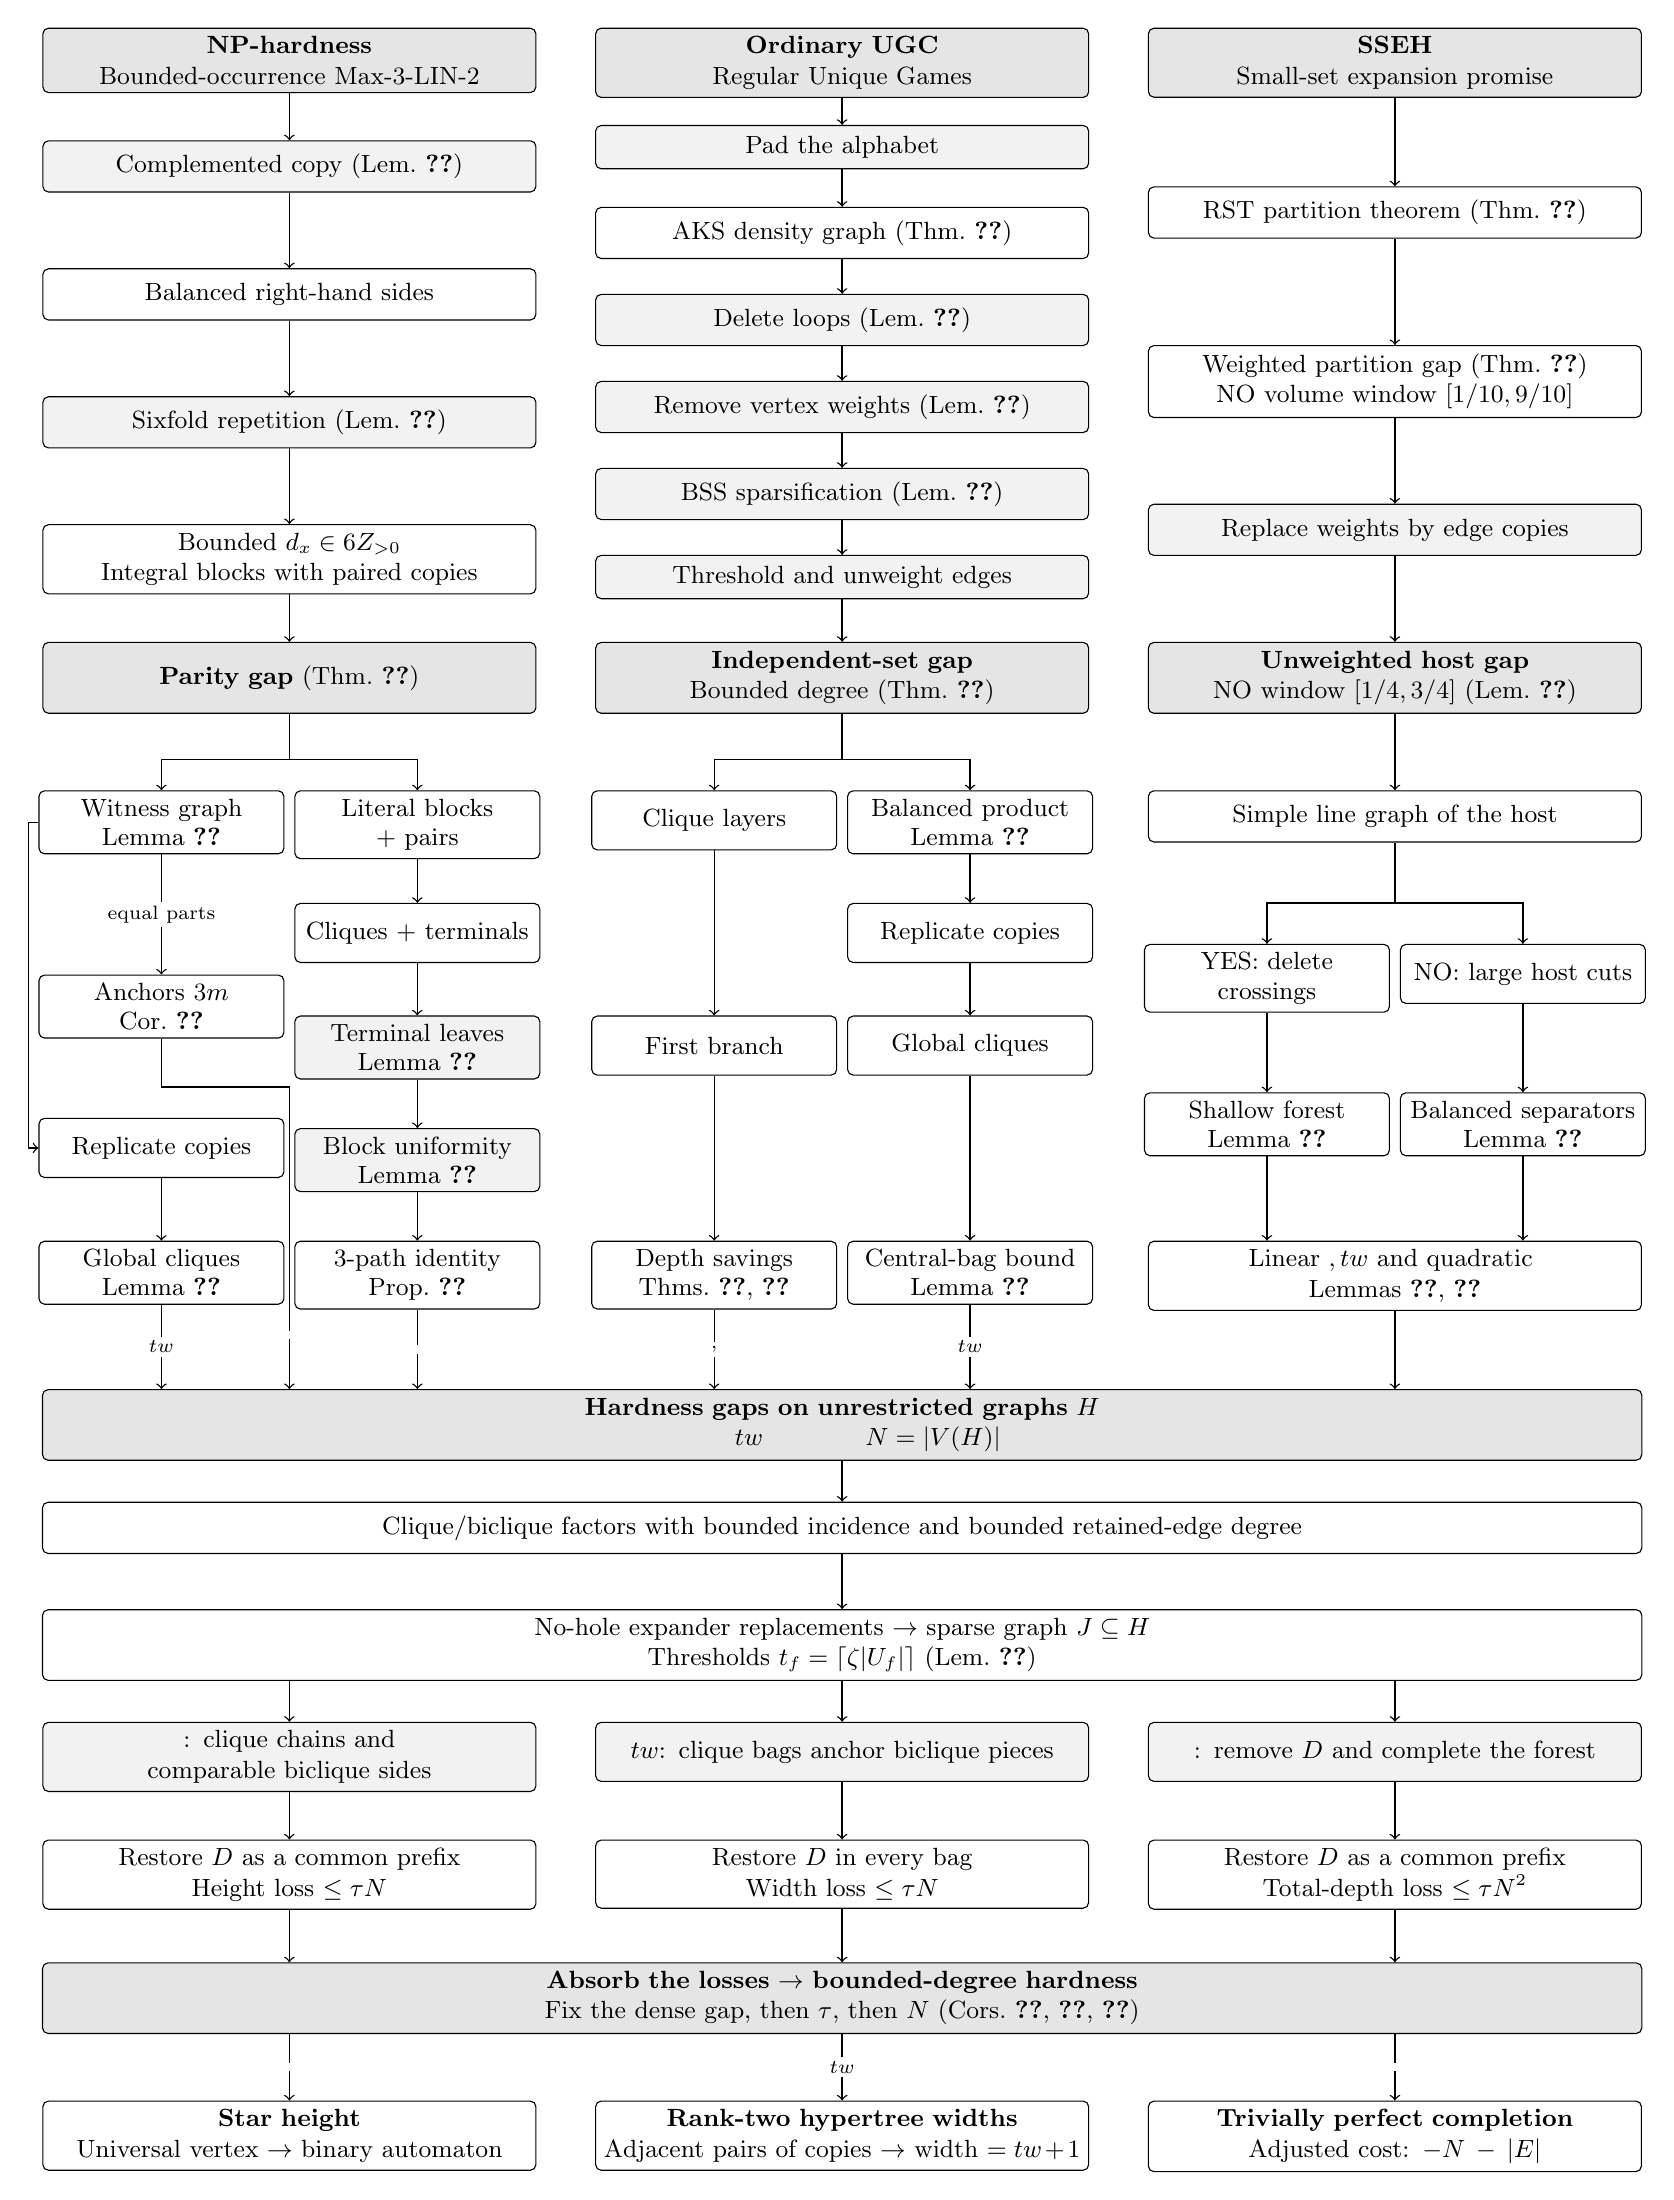
\begin{tikzpicture}[
 x=1.3cm,y=1.3cm,font=\small,
 box/.style={draw,rounded corners=2pt,align=center,text width=6.05cm,
   inner sep=3pt,anchor=north,minimum height=.65cm},
 norm/.style={box,fill=black!5},
 source/.style={box,fill=black!10,minimum height=.7cm},
 half/.style={box,text width=2.9cm,font=\fontsize{9.5}{10.5}\selectfont,
   minimum height=.75cm},
 halfnorm/.style={half,fill=black!5},
 shared/.style={box,text width=20.1cm,fill=black!10},
 arrow/.style={->,line width=.5pt},
 edgelabel/.style={font=\scriptsize,fill=white,inner sep=1.5pt}
]
% SOURCE NORMALIZATIONS: keep the three assumptions in aligned columns.
\node[source] (np-source) at (0,0)
 {\textbf{NP-hardness}\\Bounded-occurrence Max-3-LIN-2};
\node[source] (ugc-source) at (5.4,0)
 {\textbf{Ordinary UGC}\\Regular Unique Games};
\node[source] (sse-source) at (10.8,0)
 {\textbf{SSEH}\\Small-set expansion promise};

\node[norm] (np-copy) at (0,-1.1)
 {Complemented copy (Lem.~\ref{lem:parity-balance})};
\node[box] (np-balance) at (0,-2.35)
 {Balanced right-hand sides};
\node[norm] (np-repeat) at (0,-3.6)
 {Sixfold repetition (Lem.~\ref{lem:parity-repetition})};
\node[box] (np-integral) at (0,-4.85)
 {Bounded \mbox{$d_x\in6\mathbb Z_{>0}$}\\Integral blocks with paired copies};
\node[source,minimum height=.9cm] (np-ready) at (0,-6.0)
 {\textbf{Parity gap} (Thm.~\ref{thm:xor-source})};

\node[norm,minimum height=.55cm] (ugc-pad) at (5.4,-.95)
 {Pad the alphabet};
\node[box] (ugc-aks) at (5.4,-1.75)
 {AKS density graph (Thm.~\ref{thm:aks-density-source})};
\node[norm] (ugc-loops) at (5.4,-2.6)
 {Delete loops (Lem.~\ref{lem:aks-loop-removal})};
\node[norm] (ugc-unweight) at (5.4,-3.45)
 {Remove vertex weights (Lem.~\ref{lem:aks-unweighting-density})};
\node[norm] (ugc-bss) at (5.4,-4.3)
 {BSS sparsification (Lem.~\ref{lem:bss-sparsification-bound})};
\node[norm,minimum height=.55cm] (ugc-threshold) at (5.4,-5.15)
 {Threshold and unweight edges};
\node[source,minimum height=.9cm] (ugc-ready) at (5.4,-6.0)
 {\textbf{Independent-set gap}\\
  Bounded degree (Thm.~\ref{thm:bounded-degree-kr-source})};

\node[box] (sse-rst) at (10.8,-1.55)
 {RST partition theorem (Thm.~\ref{thm:rst-partition})};
\node[box] (sse-weighted) at (10.8,-3.1)
 {Weighted partition gap (Thm.~\ref{thm:sse-source})\\NO volume window $[1/10,9/10]$};
\node[norm] (sse-round) at (10.8,-4.65)
 {Replace weights by edge copies};
\node[source,minimum height=.9cm] (sse-ready) at (10.8,-6.0)
 {\textbf{Unweighted host gap}\\
  NO window $[1/4,3/4]$ (Lem.~\ref{lem:sse-unweighted-gap})};

\foreach \a/\b in {
 np-source/np-copy,np-copy/np-balance,np-balance/np-repeat,
 np-repeat/np-integral,np-integral/np-ready,
 ugc-source/ugc-pad,ugc-pad/ugc-aks,ugc-aks/ugc-loops,
 ugc-loops/ugc-unweight,ugc-unweight/ugc-bss,ugc-bss/ugc-threshold,
 ugc-threshold/ugc-ready,
 sse-source/sse-rst,sse-rst/sse-weighted,
 sse-weighted/sse-round,sse-round/sse-ready}
 \draw[arrow] (\a.south) -- (\b.north);

% NP: the shared witness graph branches to td and tw. Total depth is separate.
\node[half] (np-witness) at (-1.25,-7.45)
 {Witness graph\\Lemma~\ref{lem:xor-cover}};
\node[half] (np-pairs) at (1.25,-7.45)
 {Literal blocks + pairs};
\node[half] (np-anchors) at (-1.25,-9.25)
 {Anchors $3m$\\Cor.~\ref{cor:max-part-anchor}};
\node[half] (np-replicate) at (-1.25,-10.65)
 {Replicate copies};
\node[half] (np-cliques) at (-1.25,-11.85)
 {Global cliques\\Lemma~\ref{lem:tw-replication}};
\node[half] (np-terminals) at (1.25,-8.55)
 {Cliques + terminals};
\node[halfnorm] (np-leaves) at (1.25,-9.65)
 {Terminal leaves\\Lemma~\ref{lem:np-total-depth-added-vertices}};
\node[halfnorm] (np-blocks) at (1.25,-10.75)
 {Block uniformity\\Lemma~\ref{lem:total-depth-cover-normalization}};
\node[half] (np-paths) at (1.25,-11.85)
 {$3$-path identity\\Prop.~\ref{prop:np-total-depth-parity-identity}};
\draw[arrow] (np-ready.south) -- (0,-7.15) -| (np-witness.north);
\draw[arrow] (0,-7.15) -| (np-pairs.north);
\draw[arrow] (np-witness.south) -- node[edgelabel] {equal parts} (np-anchors.north);
\draw[arrow] (np-witness.west) -- (-2.55,0 |- np-witness.west)
 -- (-2.55,0 |- np-replicate.west) -- (np-replicate.west);
\draw[arrow] (np-replicate.south) -- (np-cliques.north);
\foreach \a/\b in {np-pairs/np-terminals,np-terminals/np-leaves,
 np-leaves/np-blocks,np-blocks/np-paths}
 \draw[arrow] (\a.south) -- (\b.north);

% UGC: layers for td/totd, a balanced product and replication for tw.
\node[half] (ugc-layers) at (4.15,-7.45)
 {Clique layers};
\node[half] (ugc-product) at (6.65,-7.45)
 {Balanced product\\Lemma~\ref{lem:multipartite-product}};
\node[half] (ugc-replicate) at (6.65,-8.55)
 {Replicate copies};
\node[half] (ugc-first) at (4.15,-9.65)
 {First branch};
\node[half] (ugc-cliques) at (6.65,-9.65)
 {Global cliques};
\node[half] (ugc-savings) at (4.15,-11.85)
 {Depth savings\\Thms.~\ref{thm:ugc-structural}, \ref{thm:total-depth-structural}};
\node[half] (ugc-bag) at (6.65,-11.85)
 {Central-bag bound\\Lemma~\ref{lem:tw-central-bag}};
\draw[arrow] (ugc-ready.south) -- (5.4,-7.15) -| (ugc-layers.north);
\draw[arrow] (5.4,-7.15) -| (ugc-product.north);
\foreach \a/\b in {ugc-layers/ugc-first,ugc-first/ugc-savings,
 ugc-product/ugc-replicate,ugc-replicate/ugc-cliques,ugc-cliques/ugc-bag}
 \draw[arrow] (\a.south) -- (\b.north);

% SSE: one line graph, separate completeness and soundness chains.
\node[box] (sse-line) at (10.8,-7.45)
 {Simple line graph of the host};
\node[half] (sse-cross) at (9.55,-8.95)
 {YES: delete crossings};
\node[half] (sse-cut) at (12.05,-8.95)
 {NO: large host cuts};
\node[half] (sse-forest) at (9.55,-10.4)
 {Shallow forest\\Lemma~\ref{lem:sse-complete}};
\node[half] (sse-separator) at (12.05,-10.4)
 {Balanced separators\\Lemma~\ref{lem:linegraph-separators}};
\node[box,minimum height=.85cm] (sse-bounds) at (10.8,-11.85)
 {Linear $\td,\operatorname{tw}$ and quadratic $\totd$\\
  Lemmas~\ref{lem:balanced-by-td}, \ref{lem:treewidth-balanced-separator}};
\draw[arrow] (sse-ready.south) -- (sse-line.north);
\draw[arrow] (sse-line.south) -- (10.8,-8.55) -| (sse-cross.north);
\draw[arrow] (10.8,-8.55) -| (sse-cut.north);
\draw[arrow] (sse-cross.south) -- (sse-forest.north);
\draw[arrow] (sse-cut.south) -- (sse-separator.north);
\draw[arrow] (sse-forest.south) -- (sse-forest.south |- sse-bounds.north);
\draw[arrow] (sse-separator.south) -- (sse-separator.south |- sse-bounds.north);

% SHARED DEGREE REDUCTION, with explicit solution-completion vertices.
\node[shared,minimum height=.75cm] (gaps) at (5.4,-13.3)
 {\textbf{Hardness gaps on unrestricted graphs $H$}\\
  $\td$\qquad $\operatorname{tw}$\qquad $\totd$\qquad \mbox{$N=|V(H)|$}};
\draw[arrow] (np-anchors.south) -- (-1.25,-10.35) -- (0,-10.35)
 -- node[edgelabel,pos=.82] {$\td$} (0,-13.3);
\draw[arrow] (np-cliques.south) --
 node[edgelabel] {$\operatorname{tw}$} (np-cliques.south |- gaps.north);
\draw[arrow] (np-paths.south) --
 node[edgelabel] {$\totd$} (np-paths.south |- gaps.north);
\draw[arrow] (ugc-savings.south) --
 node[edgelabel] {$\td,\totd$} (ugc-savings.south |- gaps.north);
\draw[arrow] (ugc-bag.south) --
 node[edgelabel] {$\operatorname{tw}$} (ugc-bag.south |- gaps.north);
\draw[arrow] (sse-bounds.south) -- (sse-bounds.south |- gaps.north);

\node[box,text width=20.1cm] (factors) at (5.4,-14.4)
 {Clique/biclique factors with bounded incidence and bounded retained-edge degree};
\node[box,text width=20.1cm] (expanders) at (5.4,-15.45)
 {No-hole expander replacements $\to$ sparse graph \mbox{$J\subseteq H$}\\
  Thresholds \mbox{$t_f=\lceil\zeta|U_f|\rceil$} (Lem.~\ref{lem:factor-replacement})};
\node[norm,minimum height=.75cm] (td-complete) at (0,-16.55)
 {$\td$: clique chains and\\comparable biclique sides};
\node[norm,minimum height=.75cm] (tw-complete) at (5.4,-16.55)
 {$\operatorname{tw}$: clique bags anchor biclique pieces};
\node[norm,minimum height=.75cm] (total-complete) at (10.8,-16.55)
 {$\totd$: remove $D$ and complete the forest};
\node[box,minimum height=.75cm] (td-restore) at (0,-17.7)
 {Restore $D$ as a common prefix\\Height loss \mbox{$\le\tau N$}};
\node[box,minimum height=.75cm] (tw-restore) at (5.4,-17.7)
 {Restore $D$ in every bag\\Width loss \mbox{$\le\tau N$}};
\node[box,minimum height=.75cm] (total-restore) at (10.8,-17.7)
 {Restore $D$ as a common prefix\\Total-depth loss \mbox{$\le\tau N^2$}};
\node[shared,minimum height=.85cm] (bounded) at (5.4,-18.9)
 {\textbf{Absorb the losses $\to$ bounded-degree hardness}\\
  Fix the dense gap, then $\tau$, then $N$
  (Cors.~\ref{cor:td-bounded-degree}, \ref{cor:tw-bounded-degree},
  \ref{cor:total-depth-bounded-degree})};
\draw[arrow] (gaps.south) -- (factors.north);
\draw[arrow] (factors.south) -- (expanders.north);
\foreach \parameter in {td,tw,total}{
 \draw[arrow] (\parameter-complete.north |- expanders.south)
   -- (\parameter-complete.north);
 \draw[arrow] (\parameter-complete.south) -- (\parameter-restore.north);
 \draw[arrow] (\parameter-restore.south)
   -- (\parameter-restore.south |- bounded.north);
}

% Only the main applications, with the essential objective adjustments.
\node[box,minimum height=.85cm] (star) at (0,-20.25)
 {\textbf{Star height}\\Universal vertex $\to$ binary automaton};
\node[box,minimum height=.85cm] (hypertree) at (5.4,-20.25)
 {\textbf{Rank-two hypertree widths}\\Adjacent pairs of copies $\to$ width $=\operatorname{tw}+1$};
\node[box,minimum height=.85cm] (completion) at (10.8,-20.25)
 {\textbf{Trivially perfect completion}\\Adjusted cost: $\totd-N-|E|$};
\draw[arrow] (star.north |- bounded.south) --
 node[edgelabel] {$\td$} (star.north);
\draw[arrow] (hypertree.north |- bounded.south) --
 node[edgelabel] {$\operatorname{tw}$} (hypertree.north);
\draw[arrow] (completion.north |- bounded.south) --
 node[edgelabel] {$\totd$} (completion.north);
\end{tikzpicture}
}
\caption{The reduction map. Shaded intermediate nodes mark normalizations.
Arrows show transformations and proof implications.}
\label{fig:introduction-reduction-map}
\end{figure}
